\documentclass{article}
\usepackage{amsmath, graphicx, amsfonts, caption, subfig, keyval}
\usepackage[numbers]{natbib}
\usepackage{xcolor}
\usepackage{hyperref}
\usepackage[boxruled,procnumbered, linesnumbered]{algorithm2e}
\usepackage[margin=1in]{geometry}
\usepackage{setspace}
\onehalfspacing
\usepackage{csquotes}

\captionsetup{justification=centering}
\newcommand{\R}{\mathbb{R}}
\newcommand{\Rr}{\mathcal{R}}
\newcommand{\D}{\mathcal{D}}
\newcommand{\C}{\mathcal{C}}
\newcommand{\X}{\mathcal{X}}
\DeclareMathOperator*{\argmin}{\arg\!\min}

\doublespacing
\makeatletter
\newcommand*{\toccontents}{\@starttoc{toc}}
\makeatother


% for the code & figure placement
\usepackage{minted}
\usemintedstyle{pastie}
\usepackage{float}
\floatplacement{figure}{H} % force figures to be placed always at defined position!

\begin{document}
\title{\Huge AM207 Final Project \\ \Large A dive into Bayesian Weather Modelling}
\singlespacing
\author{
  Victor Lei\\
           \small Institute for Applied Computational Science\\
	\small 52 Oxford Street\\
	\small Cambridge, MA\\
  \texttt{vlei@g.harvard.edu }
  \and
   Charles Liu\\
           \small Institute for Applied Computational Science\\
	\small 52 Oxford Street\\
	\small Cambridge, MA\\
  \texttt{cliu02@g.harvard.edu}
  \and
  Leonhard Spiegelberg\\
         \small Institute for Applied Computational Science\\
	\small 52 Oxford Street\\
	\small Cambridge, MA\\
 \texttt{spiegelberg@g.harvard.edu}
 \and
   Vinay Subbiah\\
         \small Institute for Applied Computational Science\\
	\small 52 Oxford Street\\
	\small Cambridge, MA\\
 \texttt{vinaysubbiah@g.harvard.edu}
}
\maketitle
\doublespacing
\begin{abstract}
Statistcal weather modelling has a long tradition. In this project we apply different methods in a Bayesian context on historical weather data. Using a simplistic approach we implement and test Bayesian models based on a network topology (Bayesian Networks) and time series based models on weather measures like temperature, pressure or precipitation. In another modelling approach we investigate a hidden markov model on weather events like rain, snow or fog. Statistical Inference based on this models has a wide range of possible applications. In this project we try to infer values for either missing data points (i.e. when measurements are not sufficient) or for missing stations / points.
\end{abstract}

\vfill
\singlespacing
\begin{center}
\bfseries\contentsname
\end{center}
\toccontents
\clearpage

\doublespacing
%%%%%%%%%%%%%%%%%%%%%%%%%%%%%%%%%%%%%%%%%%%%%%%%%%%%
%%-------------------------------                              Introduction                               -------------------------------%%
%%%%%%%%%%%%%%%%%%%%%%%%%%%%%%%%%%%%%%%%%%%%%%%%%%%%
\section{Introduction}
Traditional local and global weather modelling hugely relies on numerical simulations as well as statistical techniques. With the development and increasing popularity of Machine Learning algorithms in a Bayesian context, this project aims at serving as a study of techniques demonstrated along examples on how Bayesian techniques could be used for a data based approach in weather modelling.
\\
\\
Usually, weather data is collected at fixed weather stations that do not follow any particular pattern in terms of position or location. Hence, data is inherently spatially aware but not for every location data is available. Traditional approaches to infer missing data for specific locations rely either on numerical simulation results (and interpolating them) or on a local numerical simulation on a locally fine-grained grid. However, for many applications it is sufficient to use a statistical weather generator\cite{stochwg} which then can be used to infer a local distribution for weather parameters. One application of this could be for example to compute the risk of heavy rain for a location where no historical weather data is available. Another would be to actually use a statistical weather generator to construct initial boundary conditions of missing points that are then fed into a numerical model.
\\
\\
For this project we collected historical data of $18$ stations from $1960$-$2015$ around Boston from \url{wunderground.com}. 
\begin{figure}
\centering
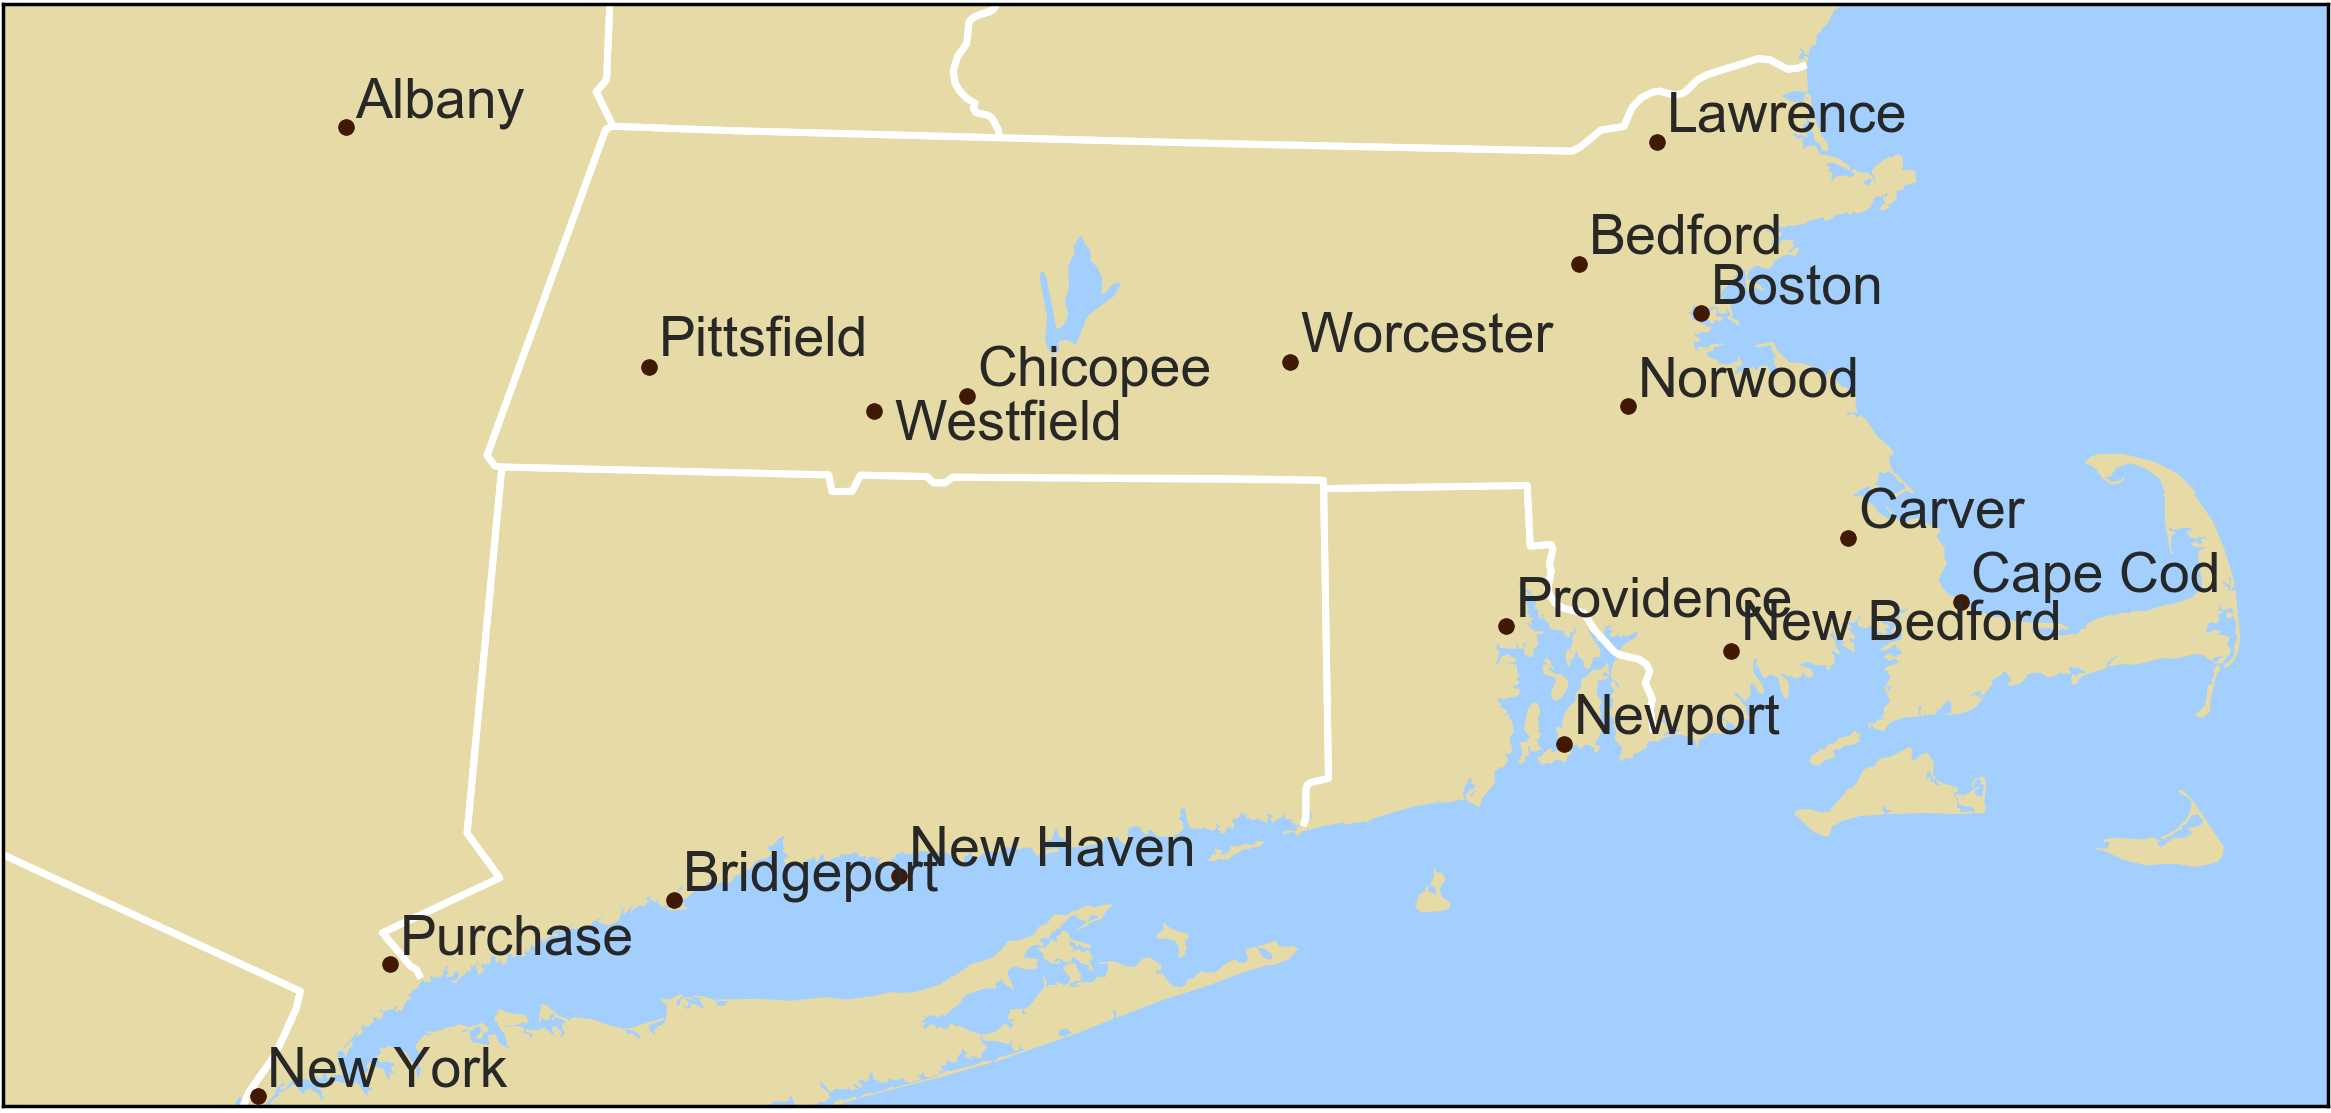
\includegraphics[scale=0.5]{../images/top_stations.png}
\caption{Illustration of the $18$ stations which data has been used for this project with weather stations being located next to airports.}
\end{figure}
Since historical weather data is usually hard to get or hidden behind paywalls, though we secured a decent amount of variables
% (Max TemperatureF,Mean TemperatureF,Min TemperatureF,Max Dew PointF,MeanDew PointF,Min DewpointF,Max Humidity, Mean Humidity, Min Humidity, Max Sea Level PressureIn, Mean Sea Level PressureIn, Min Sea Level PressureIn, Max VisibilityMiles, Mean VisibilityMiles, Min VisibilityMiles, Max Wind SpeedMPH, Mean Wind SpeedMPH, Max Gust SpeedMPH,PrecipitationIn, CloudCover, Events, WindDirDegrees)
we do not claim that our data base should be used for a real-world application. Instead, it serves more as a base for applying several techniques and investigating their feasibility.
\\
\label{sec:intro}
\section{Bayesian Networks}
\subsection{Network construction}
Leo
\subsubsection{Initial Ordering}
Leo
\subsubsection{K2 algorithm}
Charles
\subsection{Inference}
\subsubsection{Direct Sampling}
Charles your call
\subsubsection{Monte Carlo / Gibbs Sampling}
Leo
\subsection{Application}
Charles again


%% print out bib
\onehalfspacing
\bibliographystyle{plainnat}
\bibliography{bibliography}

\end{document}